% !TeX root = ../main.tex
% Add the above to each chapter to make compiling the PDF easier in some editors.

\chapter{Automatisierte Fahrzeuge im urbanen Raum}\label{chapter:automatisiertes Fahren}
\enquote{Die Motivation zur Teilnahme am Straßenverkehr ist Mobilität, nicht Sicherheit} \parencite[S. 146]{Huguenin.2017}. Aus dieser Anforderung ergibt sich ein hoher Anspruch an automatisierte Fahrzeuge. Sie dürfen keinerlei Einschränkungen bezüglich der Mobilität mit sich bringen, um ihre Nutzer zufrieden zu stellen. Gleichzeitig müssen hohe Sicherheitsanforderungen eingehalten werden, um solche Fahrzeuge überhaupt auf den Markt bringen zu können. In diesem Kapitel werden Fahrsituationen für menschliche Fahrer, die in Kapitel \ref{section:Zuordnung der Unfälle zu Fahrsituationen} mit der Risiko-Kategorie \textit{c} oder höher bewertet wurden, mit denen für automatisierte Fahrzeuge verglichen. Kapitel \ref{section:Allgemeines} gibt zunächst einen Überblick über verschiedene Automatisierungsgrade und Fahrerassistenzsysteme. Anschließend werden in Kapitel \ref{section:Vergleich menschlicher Fahrer automatisierte Systeme} urbane Fahrsituationen miteinander verglichen, um herauszufinden, ob sich das Risiko, das Fahrsituationen mit menschlichen Fahrern einhergeht, bei automatisierten Systemen verändert.

\section{Allgemeines}\label{section:Allgemeines}
Dieses Kapitel gibt einen kurzen Überblick über die verschiedenen Stufen der Automatisierungsgrade und über verschiedene Fahrerassistenzsysteme. Die FAS werden berücksichtigt, da eine Zusammenführung bestehender Assistenzsysteme zum automatisierten Fahren das wahrscheinlich größte Potential bietet.

\subsection{Klassifizierung automatisierter Fahrfunktionen}
Automatisierte Fahrfunktionen können in fünf Stufen unterteilt werden. Der Automatisierungsgrad nimmt dabei mit jeder Stufe zu. Betrachtet man die Klassifizierung der automatisierten Fahrfunktionen nach \ac{BASt}, werden Fahrten oder Situationen, bei denen kein in die Längs- oder Querführung eingreifendes System aktiv ist, der Stufe 0 zugeordnet. Alle fünf Stufen werden in Tabelle \ref{tab:Automatisierungsgrad} erläutert.

\begin{table}[htpb]
	\scriptsize
	\caption[Benennung und Klassifizierung automatisierter Fahrfunktionen]{Benennung und Klassifizierung automatisierter Fahrfunktionen \parencite[S. 3]{Gasser.2011}}\label{tab:Automatisierungsgrad}
	\centering
	\begin{tabular}{l p{3cm} p{10cm}}
		\toprule
		Stufe & Nomenklatur & Beschreibung Automatisierungsgrad und Erwartung des Fahrers \\
		\midrule
		0 & Nur Fahrer & Fahrer führt dauerhaft die Längsführung und die Querführung aus. \\
		1 & Assistiert & Fahrer führt dauerhaft \underline{entweder} die Quer- \underline{oder} die Längsführung aus. Die jeweils andere Fahraufgabe wird in gewissen Grenzen vom System ausgeführt. \\
		2 & Teilautomatisiert & Das System übernimmt Quer- \underline{und} Längsführung (für einen gewissen Zeitraum und/oder in spezifischen Situationen). \\
		3 & Hochautomatisiert & Das System übernimmt Quer- und Längsführung für einen gewissen Zeitraum in spezifischen Situationen. \\
		4 & Vollautomatisiert & Das System übernimmt Quer- und Längsführung vollständig in einem definierten Anwendungsfall. \\
		\bottomrule
	\end{tabular}
\end{table}

Der Unterschied zwischen Stufe 2 und 3 besteht darin, dass der Fahrer in Stufe 3 das System nicht dauerhaft überwachen muss. Er wird bei Bedarf zur Übernahme der Fahraufgabe mit ausreichender Zeitreserve aufgefordert. Stufe 4 bezieht sich lediglich auf einen definierten Anwendungsfall. Das autonome Fahren stellt eine weitere (letzte) Entwicklungsstufe dar. Laut \Textcite[S. 34]{Maurer.2015} werden beim autonomen Fahren alle Aufgaben des Drei-Ebenen-Models (Navigation, Führung und Stabilisierung) vollautomatisiert ausgeführt. Diese Definition wird erweitert um die Annahme, dass die Ausführung der Fahraufgabe auf Basis maschinell autonomen Verhaltens, innerhalb eines vorher festgelegten Verhaltensrahmens, geschieht.

Mit der Zunahme des Automatisierungsgrads steigen nicht nur die technischen Anforderungen sondern auch die der Kunden und der öffentlichen Hand. Dies erschwert den Entwicklungsprozess zunehmend, da sich diese Anforderungen zum Teil widersprechen. Während sich der Kunde Fahrspaß, Sicherheit als Serienausstattung und klare Systemgrenzen wünscht, stehen für die öffentliche Hand das Senken der Unfall- und Opferzahlen sowie geringe Infrastrukturinvestitionen im Vordergrund. Der Hersteller muss diese Punkte weitestgehend erfüllen und hat zusätzlich eigene Ansprüche wie Wettbewerbsdifferenzierung oder geringe Herstellungskosten \parencite[S. 8]{Meitinger.2008}. %Noch mehr dazu oder einfach weglassen?

\subsection{Fahrerassistenzsysteme}
Es gibt verschiedene Möglichkeiten den Fahrer anhand von Assistenzsystemen zu unterstützen. \ac{IO} Systeme sind Systeme, die an markanten Punkten, z.B. an einer Kreuzung, installiert werden. Diese Systeme sind nicht ans Fahrzeug gebunden und daher auch nicht auf Neuerungen im  Fahrzeug angewiesen. Häufig werden sie in Form von aktiven Verkehrszeichen ausgeführt. Fahrzeugautarke Systeme stellen Systeme dar, deren Funktion weder auf Komponenten in der Kreuzung noch auf Systeme in anderen Fahrzeugen angewiesen sind. Zur Umfelderfassung werden Sensoren im Fahrzeug benötigt, die Informationen über Vorfahrtsregelungen werden aus GPS mit digitalen Karten oder Kamerasystemen gewonnen. Die \ac{V2V} Kommunikation funktioniert nur zwischen damit ausgestatteten Fahrzeugen, kann dafür z.B. bei eingeschränkten Sichtbereichen an Kreuzungen besser agieren. Kooperative Systeme können Systemkomponenten der Infrastruktur mit Elementen im Fahrzeug kombinieren. Das Fahrzeug kann so beispielsweise Informationen zum Phasenwechsel einer LSA erhalten \parencite[S. 23-26]{Mages.2008}. Die genannten Möglichkeiten werden bei der Entwicklung nicht nacheinander durchlaufen sondern überschneiden sich \parencite[S. 88]{WissenschaflicherBeiratbeimBundesministerfurVerkehrBauundStadtentwicklung.2011}.

Der Vorteil von Kommunikationslösungen besteht darin, dass die Anforderungen an die \enquote{konventionelle} Umfeldsensorik sinken. Des weiteren wird die räumliche und zeitliche Wahrnehmung erweitert. So ist es möglich, Verkehrsunfälle zu verhindern, indem eine mögliche Gefahrensituationen im Voraus erkannt wird \parencite[S. 59]{Gerstenberger.17.02.2015}. Ein weiterer Vorteil ist, dass mögliche Gefahren trotz eventueller Sichtbehinderungen frühzeitig erkannt werden. Nachteilig ist hingegen, dass alle Fahrzeuge eine gewisse Mindestausrüstung enthalten müssen, um den Anforderungen gerecht zu werden \parencite[S. 2]{Mages.2008}.

Die Assistenzsysteme selbst können in vier Gruppen unterteilt werden: Informationssysteme, Warnsysteme, aktiv unterstützende Systeme und eingreifende Systeme. Laut \Textcite[S. 11]{Meitinger.2008} ist die Wirksamkeit von eingreifenden Systemen am höchsten einzuschätzen. Eine Erweiterung um eine fünfte Gruppe würde dann Systeme darstellen, die selbständig bestimmte Aktionen übernehmen, ohne dass der Fahrer dies verhindern oder korrigieren kann \parencite[S. 13]{Vollrath.2006}. Bei der Wirkung von FAS wird zwischen der spezifischen und der unspezifischen Wirkung unterschieden. Während Auswirkungen, die sich aus Reaktionen des Fahrers auf Informationen, Warnungen und Eingriffe ergeben, als spezifisch bezeichnet werden sind Effekte, die sich auf die Fahrweise auswirken, unspezifisch \parencite[S. 50f]{Grundl.2005}.

\enquote{Ziel eines Aktiven Sicherheitssystems ist die Verbesserung der Verkehrssicherheit. Wie groß der Sicherheitsgewinn ist hängt von der Anzahl der relevanten Situationen, die in einem betrachteten Zeitraum auftreten, der Wirksamkeit des Systems, seiner konstruktiven Sicherheit und dem Schutz gegen Missbrauch ab} \parencite[S. 10]{Meitinger.2008}. Es besteht jedoch immer die Gefahr, dass sich der Fahrer durch das System sicherer fühlt und aufgrund dessen ein höheres Risiko eingeht. Hierdurch wird die ursprüngliche Verbesserung des Sicherheitssystems wieder aufgehoben. Aktive Sicherheitssysteme sind effizienter, wenn sie gezielt gegen Unfalltypen, die häufig auftreten, wirken. Hierfür ist die absolute Anzahl der Unfälle von Bedeutung \parencite[S. 19]{Meitinger.2008}.

Nach \Textcite[S. 10]{Blakaj.14.09.2016} besteht ein \ac{FAS} aus drei Grundkomponenten:

\begin{itemize}
	\item Sensorik (zuständig für die Informationserkennung)
	\item Hard- und Software (verarbeitet die durch die Sensoren erfassten Informationen und gleicht diese mit dem Soll-Zustand ab)
	\item Aktorik oder auch Mensch-Maschine Schnittstelle genannt (gleicht den Unterschied zwischen dem Ist- und Soll-Zustand aus).
\end{itemize}

Bei der Sensorik werden Videokameras verwendet, um die Fahrbahn zu beobachten. Radar- oder Lasersensoren dienen der Abstands- und Geschwindigkeitserkennung \parencite[S. 4f]{Schmidt.2010}. Die dritte Komponente würde sich beim voll automatisierten Fahren ändern. Der Mensch ist nicht mehr dafür verantwortlich, Abweichungen vom Soll-Zustand auszugleichen. Es kann sogar zu Fahrten kommen (z.B. Parkplatzsuche), bei denen gar kein Fahrer an Bord ist.

In Abbildung \ref{fig:FAS} werden \ac{FAS} dargestellt, die sich bereits auf dem Markt befinden oder noch in der Entwicklung sind. Es muss berücksichtigt werden, dass die Übersicht aus dem Jahr 2006 ist. Es kann also durchaus sein, dass Systeme, die sich damals noch in der Entwicklung befanden inzwischen auf dem Markt sind. Die Abbildung wurde gewählt, weil darin nicht nur die einzelnen \ac{FAS} genannt werden sondern auch die Ebenen, in denen sie eingreifen (Stabilisierungs- oder Führungsebene).

Des weiteren wird an einer Fußgänger- und Verkehrszeichenerkennung gearbeitet. Sie werden in Abbildung \ref{fig:FAS} nicht erwähnt, haben jedoch bei Fahrsituationen im urbanen Raum eine wesentliche Bedeutung. \Textcite[S. 52]{Gschwendtner.2015} betrachtet \ac{FAS} bezüglich ihrer Wirksamkeit im niedrigen Geschwindigkeitsbereich. Er kommt zu dem Ergebnis, dass die automatische Notbremse das höchste Potential besitzt, da sie sowohl die Unfallfolgen von Unfällen mit Personen- also auch mit Sachschaden reduzieren kann. Der Kreuzungsassistent beeinflusst dagegen überwiegend Unfälle mit Personenschaden. Eine hohe Einwirkung auf Sachschadensunfälle hat die Einparkhilfe. Das Potential eines Spurwechselassistenten schätzt er in beiden Bereichen eher gering ein. Am ehesten können jedoch Sachschäden reduziert werden.

\begin{savenotes}
	\begin{figure}[H]
		\centering
		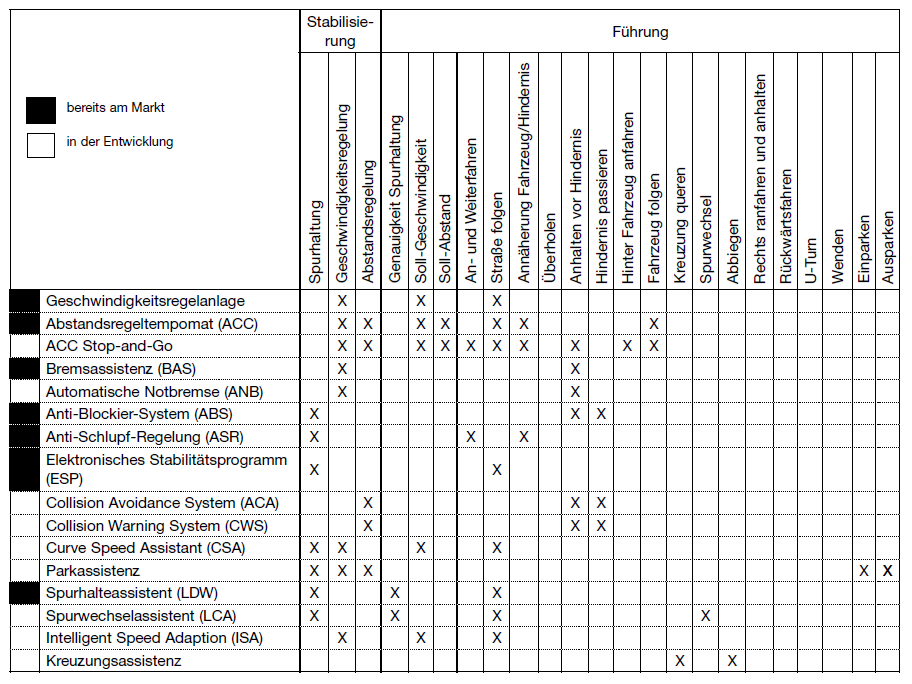
\includegraphics[width=15cm,height=11.25cm]{figures/FAS}
		\caption[Klassifikation von Assistenzsystemen im Hinblick auf ihre Funktionalität auf der Stabilisierungs- und Führungsebene]{Klassifikation von Assistenzsystemen im Hinblick auf ihre Funktionalität auf der Stabilisierungs- und Führungsebene \parencite[S. 31]{Vollrath.2006}}\label{fig:FAS}
	\end{figure}
\end{savenotes}

Obwohl Systeme, die bei niedrigen Geschwindigkeiten wirken (z.B. Einparkhilfe), ein hohes Potential zur Unfallvermeidung mit sich bringen, werden sie aktuell häufig als Komfortsysteme vermarktet, da sie nur einen indirekten Einfluss haben. Dies liegt daran, dass es erst wenige Systeme gibt, die nicht nur warnen, sondern direkt eingreifen. Auffällig ist zudem, dass bei allen vorhandenen \ac{FAS} die Fahrzeugflanken, bei denen es bei einer Beschädigung zu hohen Reparaturkosten kommt, vernachlässigt werden. Dies sollte in Zukunft durch eine Rundumüberwachung vermieden werden. Zudem erhofft man sich zukünftig, z.B. von Valet-Parking-Systemen oder FAS-Systemen, die vom Nutzer gesteuert werden (z.B. Handysteuerung), weitere Verbesserungen im Bereich der Sachschadensunfälle \parencite[S. 18-21]{Gschwendtner.2015}.

\Textcite[S. 2]{Schendzielorz.21.09.2016} arbeitet an der Entwicklung eines Kreuzungsassistenten. Dieser prüft mit Hilfe von \ac{V2I} und \ac{V2V}-Kommunikation plus entsprechenden infrastrukturseitigen Einrichtungen, ob der Fahrer vor einer Konfliktsituation an Knoten gewarnt werden muss. Die Knotenpunkte werden mit Laserscannern, die auf Ampel- oder Lichtmasten montiert sind, aus der Vogelperspektive betrachtet. Der Fokus liegt hierbei auf den Szenarien Rotlichtverstoß, Links- und Rechtsabbiegen.

\Textcite[S. 224-230]{Grundl.2005} betrachtet in seiner Arbeit Unfälle, die durch eine Verkehrszeichenerkennung vermeidbar gewesen wären. Er geht auf die Erkennung von Ampeln mit Rotlicht, Stoppschilder, Vorfahrt-gewähren-Schilder und Richtungsgebot-Schilder ein. Kritisch betrachtet er vor allem die Erkennung des Ampellichts, da Sensoren die dies zuverlässig ermöglichen noch sehr kostspielig sind. Zudem muss berücksichtigt werden, dass ein Verkehrszeichen oft absichtlich nicht befolgt wird, was die Wirksamkeit eines \ac{FAS} in diesem Bereich deutlich reduziert.

Zusätzlich zur Verkehrszeichenerkennung befasst sich \Textcite[S. 239-246]{Grundl.2005} mit der Gestaltung eines Spurwechselassistenten. Er kommt zu dem Schluss, dass der Totewinkel nicht entscheidend für die Vermeidung von Unfällen beim Spurwechsel ist. Ausschlaggebend ist die Erkennung von Fahrzeugen, die sich mit hoher Geschwindigkeit von hinten nähern. Dies gilt hauptsächlich für Fahrsituationen auf der Autobahn. Im urbanen Raum könnten Unfälle beim Spurwechsel vermieden werden, indem nicht nur der vor dem Fahrzeug liegende Bereich sondern ebenso die seitlichen Bereiche des Fahrzeugs erfasst werden. Von der Seite nahende Gefahren könnten so besser erkannt und bestenfalls vermieden werden.

\subsection{Rechtlichehintergründe}
Um fahrerloses Fahren zu ermöglichen muss das aktuell geltende Recht angepasst werden. Nach der heutigen Rechtslage würde der Fahrer schon bei Hoch- bzw. Vollautomatisierung, in den Phasen die autonom gesteuert werden, gegen seine Pflichten aus der StVO verstoßen. Sie gibt an, dass der Fahrer jederzeit in der Lage sein muss in das Verkehrsgeschehen eingreifen zu können. Ziel der Vollautomatisierung ist jedoch, dass der Fahrer sich während der Fahrt anderen Aufgaben widmen kann und nicht permanent den Fahrtverlauf überwachen muss oder Fahrzeuge Strecken ganz ohne Fahrer zurücklegen können. Die Nutzung von Hoch- bzw. Vollautomatisierung ist somit bereits nicht mehr als zulässig einzustufen, weil sie eine Abwendung des Fahrers von seiner Fahraufgabe vorsehen. Die Haftung des Fahrzeughalters bleibt dagegen widerspruchsfrei auf die höheren Automatisierungsgrade anwendbar. Bei der Produkthaftung ergibt sich bei einer automatisierten Fahrt, dass jeder Schaden, der nicht auf das Fehlverhalten eines Dritten zurückzuführen ist, potentiell zu einem Fall von Produkthaftung führt. Das könnte für die Hersteller enorme Folgen haben. Hier muss also zusätzlich nach Lösungen gesucht werden \parencite[S. 6f]{Gasser.2011}. Auch \Textcite[S. 8]{Mages.2008} stellt fest, dass nicht vom Fahrer übersteuerbare Systeme grundlegende Änderungen des Straßenverkehrsrechts erfordern. Systeme mit erheblichem unfallvermeidendem oder schützendem Potential, die nicht übersteuerbar sind, können aktuell auch nicht unter realen Bedingungen getestet werden. Es sollte daher geprüft werden, ob eine besondere Form der Typgenehmigung möglich ist, die die Risiken der Erprobung unter realen Bedingungen für die Herstelle, Halter und Versicherungen kalkulierbar macht \parencite[S. 89]{WissenschaflicherBeiratbeimBundesministerfurVerkehrBauundStadtentwicklung.2011}. 

\section{Vergleich menschlicher Fahrer automatisierte Systeme}\label{section:Vergleich menschlicher Fahrer automatisierte Systeme}
\enquote{Ein enormes Potenzial, Verkehrsunfälle deutlich zu reduzieren bietet das automatisierte Fahren. Über 90 Prozent aller Unfälle sind heute auf menschliches Fehlverhalten zurückzuführen. Mit dem Einzug von Fahrcomputern werden wir die Fahrer deutlich entlasten und kritische Verkehrssituationen massiv reduzieren. Der Sprung zum automatisierten und vernetzten Fahren ist damit nicht nur die größte Mobilitätsrevolution seit der Erfindung des Automobils, sondern bringt auch ein großes Plus an Sicherheit} \parencite[S. 4]{DEKRA.2017}. In der Unfallstatistik ist zu erkennen, dass Fahrerassistenzfunktionen und sicherheitsrelevante Funktionen in Fahrzeugen bereits einen Beitrag zur Sicherheit im Straßenverkehr leisten. Ein Beispiel ist das von Bosch entwickelte elektronische \ac{ABS} oder das Elektronische Stabilitätsprogramm \acs{ESP} von Mercedes \parencite[S. 4]{Hillenbrand.2012}.

\begin{table}[htpb]
	\scriptsize
	\caption[Stärken und Schwächen von Mensch und Maschine]{Stärken und Schwächen von Mensch und Maschine \parencite[S. 147]{Huguenin.2017} }\label{tab:Mensch vs. Maschine}
	\centering
	\begin{tabular}{l p{5cm} p{7cm}}
		\toprule
		Systemelement & Stärken & Schwächen \\
		\midrule
		\enquote{Mensch} & - flexibles situationsbezogenes Denken & - Körperlich und psychisch bedingte Leistungsschwankungen \\
		 & - Antizipationsfähigkeit & - Emotionalität \\
		 & - Vielseitigkeit & - Beeinfluss- und Ablenkbarkeit \\
		\midrule		 
		\enquote{Maschine} & - Konstanz & - unflexibel, programmiert \\
		 & - Zuverlässigkeit & - mangelhafte Fehlerdetektion \\
		 & - Geschwindigkeit & - spezialisiert, wenig vielseitig \\		 
		\bottomrule
	\end{tabular}
\end{table}

Es darf jedoch nicht vernachlässigt werden, dass eine hohe Zahl an Unfällen fälschlicherweise dem Menschen zugeordnet wird. \Textcite[S. 147]{Huguenin.2017} betont, dass das eingesetzt System auch mangelhaft sein kann. In Tabelle \ref{tab:Mensch vs. Maschine} werden die Stärken und Schwächen von Mensch und Maschine gegenübergestellt. \Textcite[S. 5]{Gasser.2011} erwähnt, dass einige wenige Unfallkonstellationen sich auch durch die Erhöhung des Automatisierungsgrades nicht verhindern lassen. Er stellt die Wirkung der Fahrzeugautomatisierung bildlich dar (Abbildung \ref{fig:Wirkung_Fahrzeugautomatisierung}). Hier ist zu erkennen, dass die erhoffte Wirkung unter Umständen relativ gering ausfällt.

\begin{savenotes}
	\begin{figure}[H]
		\centering
		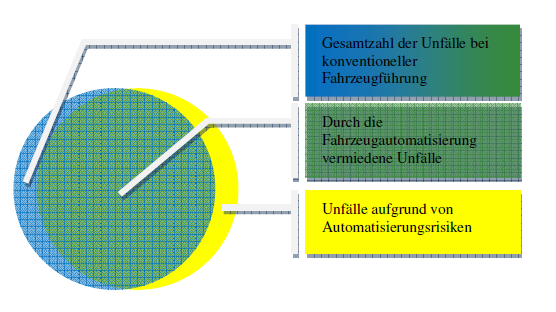
\includegraphics[width=10.7cm,height=6cm]{figures/Wirkung_Fahrzeugautomatisierung}
		\caption[Wirkung der Fahrzeugautomatisierung]{Wirkung der Fahrzeugautomatisierung nach \Textcite[S. 5]{Gasser.2011}}\label{fig:Wirkung_Fahrzeugautomatisierung}
	\end{figure}
\end{savenotes}

Im folgenden Kapitel werden die menschlichen Fahrsituationen aus Kapitel \ref{subsection:Zuordnung mit den aufgenommenen Fahrsituationen} mit automatisierten verglichen. 

\section{Vergleich der Fahrsituationen innerhalb des Testgebiets}\label{section:Fahrsituationen im Vergleich}
Ziel dieses Kapitels ist es herauszufinden, welche, im Testgebiet aufgenommenen, Situationen  mit automatisierten Fahrzeugen einfacher bewältigt werden können und in welchen sie evtl. an Grenzen stoßen.
Um die menschlichen Fahrsituationen besser mit automatisierten vergleichen zu können werden sechs Bereiche gebildet, die verschiedene Probleme darstellen. Diese werden in Tabelle \ref{tab:Cluster} aufgezählt. Die Fahrsituationen mit der Risikokategorie \textit{c} oder höher werden anschließend den jeweiligen Bereichen zugeordnet. 

\begin{table}[htpb]
	\scriptsize
	\caption[Cluster zum Vergleich zwischen meschl. und automatisierten Fahrsituationen]{Cluster zum Vergleich zwischen meschl. und automatisierten Fahrsituationen}\label{tab:Cluster}
	\centering
	\begin{tabular}{l l}
		\toprule
		Nummer & Beschreibung \\
		\midrule
		1 & Einfaches menschliches Versagen \\
		2 & Menschliches Versagen in komplexen Situationen \\
		3 & Sichtbehinderungen \\
		4 & Kommunikation zwischen den Verkehrsteilnehmern \\
		5 & Grenzen automatisierter Systeme \\
		6 & Sonstiges \\		 
		\bottomrule
	\end{tabular}
\end{table}

\subsubsection{Einfaches menschliches Versagen}
Es kann davon ausgegangen werden, dass die meisten Fahrsituationen, bei denen es zu Unfällen durch einfaches menschliches Versagen kommt mit automatisierten Systemen verhindert werden. In diesen Bereich fallen die Fahrsituationen, denen die Feintypen 609, 619 und 623 zugrunde liegen und bei denen es häufig zu Auffahrunfällen kommt. Diese Unfälle könnten bereits jetzt größtenteils mit einem aktiv eingreifenden Notbremsassistenten verhindert werden und sollten daher für automatisierte Systeme keine große Schwierigkeiten darstellen. Auffahrunfälle entstehen häufig durch einen zu geringen Sicherheitsabstand und Unaufmerksamkeit der menschlichen Fahrer. Automatisierte Systeme ermöglichen es, den Sicherheitsabstand so anzupassen, dass ein notwendiges Bremsmanöver aufgrund des vorausfahrenden Fahrzeugs rechtzeitig eingeleitet werden kann.

Fahrsituationen der Feintypen 631, 641, 651 und 63/64 führen zu Unfällen beim Spurwechsel bzw. nebeneinander Fahren. Diese werden ebenfalls häufig durch unaufmerksames Handeln des Fahrers ausgelöst. Bei Unfällen, die durch Fehler beim Spurwechsel entstehen, führen die Fahrzeugführer vor dem Spurwechsel häufig keinen Schulterblick oder Blick in den Rückspiegel durch. Dies führt dazu, dass herannahende oder auf gleicher Höhe befindliche Fahrzeuge übersehen werden. Um solche Situationen auf Autobahnen zu vermeiden gibt es bereits Spurwechselassistenten, diese funktionieren bis jetzt jedoch noch nicht im niedrigen Geschwindigkeitsbereich. Da die Ansätze bereits vorhanden sind müssten sich diese Konflikte mit automatisierten Fahrzeugen vermeiden lassen. Wichtig ist hierbei, dass auch der seitliche Bereich des Fahrzeugs mit Erkennungssystemen ausgestattet wird. So ist es auch Möglich auf Fehler der anderen Fahrzeugführer zu reagieren, wenn diese z.B. ihre Spur nicht einhalten oder nach einem Überholvorgang zu früh wieder einscheren, kann das automatisierte System ausweichen oder ein Bremsmanöver einleiten. Ebenso kann das geplante Manöver abgebrochen werden, wenn beide Fahrzeuge vorhaben gleichzeitig auf die selbe Spur zu wechseln. Fahrsituationen die zu Unfällen mit dem Feintyp 501 führen entstehen, wenn sich das Fahrzeug zu weit rechts befindet und deshalb der seitliche Sicherheitsabstand zu parkenden Fahrzeugen zu gering ist. Automatisierte Systeme müssten diese Unfälle vermeiden können, da sie die Spur halten oder ausweichen/bremsen, wenn ein parkendes Fahrzeug zu weit in den Straßenraum hineinragt.

Dem Feintyp 141 liegt die Fahrsituation geradeaus Fahren zugrunde. Hier kommt es zu Unfällen durch Kontrollverlust, aufgrund überhöhter Geschwindigkeit oder Ablenkung des Fahrers. Automatisierte Systeme müssen es ermöglichen, die Geschwindigkeit nicht nur an ein vorausfahrendes Fahrzeug, sondern auch an den Straßenverlauf und die Umfeldbedingungen (z.B. geringere Griffigkeit der Fahrbahn durch Nässe oder Glätte), anzupassen. Ist dies möglich können auch solche Unfälle verhindert werden. Unfälle, bei denen der Fahrer, aufgrund von Ablenkung von der Fahrbahn abkommt, fallen weg.

Unfälle die häufig zu Sachschaden führen ereignen sich vor allem bei der Fahrsituation Ein-/Ausparken in Bereichen mit Längsaufstellung. Ihnen wurde der Feintyp 701 zugeordnet. Solche Unfälle können mit automatisierten Systemen verhindert werden. Es gibt bereits Parkassistenzsysteme, diese Warnen den Fahrer jedoch größtenteils nur und greifen nicht aktiv in den Parkvorgang ein. Hier sind die Grundlagen jedoch schon geschaffen, um Unfälle beim Parken zu vermeiden.

\subsubsection{Menschliches Versagen in komplexen Situationen}
\enquote{Der Fahrer ist bei der Entstehung von Unfallsituationen häufig nicht in der Lage, ein vollständiges Situationsmodell aufzubauen und kann somit nicht angemessen auf die Situation in der Umgebung reagieren} \parencite[S. 48]{Zademach.24.09.2015}. Der Aufbau eines Situationsmodells wird durch sich potenziell bewegende Objekte erschwert, da Fahrer das Verhalten dynamischer Objekte nur schwer vorhersagen können. Fahrsituationen an Knotenpunkten sind daher besonders anspruchsvoll und führen vermehrt zu Unfällen. Im Testgebiet kam es häufig zu Konflikten zwischen Linksabbiegern und entgegenkommenden Fahrzeugen (Feintyp 211). In dieser Situation muss die Geschwindigkeit und die Entfernung des entgegenkommenden Fahrzeugs berücksichtigt werden, um entscheiden zu können, ob die vorhandene Zeitlücke ausreicht die Kreuzung zu überqueren. \Textcite[S. 9]{Mages.2008} gibt in seiner Arbeit an, dass ein automatisiertes System vielfältige Anforderungen erfüllen muss, um Unfälle an Kreuzungen vermeiden zu können. Dazu zählt die Erfassung von Kreuzungen und Vorfahrtsregelungen, das Erkennen des nächsten Phasenwechsels von LSA, die Berücksichtigung vorausfahrender Fahrzeuge und Fußgänger sowie das Abschätzen der Gefahr von Kollisionen mit dem Querverkehr. Des weiteren muss an Knotenpunkten besonders Rücksicht auf ungeschützte Verkehrsteilnehmer genommen werden, die häufig auf getrennten Anlagen geführt werden. Hier spielt laut \Textcite[S. 310]{Schreiber.2014b} die Detektion von Radfahrern, die sich mit vergleichsweise hohen Geschwindigkeiten bei oft gleichzeitig eher geringer Abbiegegeschwindigkeit des Kfz von hinten nähern, eine bedeutende Rolle. Ebenso sollten Assistenzsysteme auch links fahrende Radfahrer erkennen können, so dass auch Konflikte beim Linksabbiegen verhindert werden. Dies ist vor allem für die Fahrsituationen mit den Feintypen 243, 244 und 224 sowie 342 und 349 relevant.

Bei Unfällen die sich beim Wenden ereignen kann es auch zu Konflikten mit entgegenkommenden Fahrzeugen kommen (Feintyp 723). Hier werden an automatisierte Fahrzeuge die gleichen Anforderungen gestellt, die bereits bei den Knotenpunkten genannt wurden. Zusätzlich muss berücksichtigt werden, dass der Wendevorgang an einer Stelle eingeleitet wird, in der Wenden erlaubt ist. Ein Konflikt mit einem entgegenkommenden Fahrzeug kann sich auch außerhalb von Knotenpunkten ereignen. Bei dieser Fahrsituation (Feintyp 681) muss ein automatisiertes Fahrzeug in der Lage sein die eigene Spur zu halten. Der Straßenverlauf muss trotz entgegenkommender Fahrzeuge, die möglicherweise zur Blendung von Kameras oder Sensoren führen, zuverlässig erkannt werden. Des weiteren muss das automatisierte Fahrzeug bei möglichen Spurabweichungen des entgegenkommenden Fahrzeugs rechtzeitig reagieren können.

Fahrsituationen, bei denen es zu den Feintypen 401 und 421 kommen kann können auch zu den komplexeren gezählt werden. Hierbei treten Fußgänger entweder von links oder rechts auf die Fahrbahn. In diesem Fall muss ein automatisiertes System erkennen, dass ein Fußgänger die Absicht hat die Straße außerhalb eines Fußgängerüberwegs zu queren oder sich schon auf der Straße befindet und die Geschwindigkeit anpassen oder ein passendes Bremsmanöver einleiten. Dies sollte möglich sein, da bei diesen zwei konkreten Fahrsituationen keine Sichtbehinderung vorhanden ist, die es dem System erschwert Fußgänger zu erkennen. Zu einem Konflikt kann es jedoch kommen, wenn Fußgänger unmittelbar vor dem Fahrzeug auf die Straße treten und der erforderliche Bremsweg nicht vorhanden ist. Dieser ist bei automatisierten Fahrsituationen zwar deutlich geringer als bei menschlichen, aber trotzdem vorhanden.

Sobald ein \enquote{optimales System} vorliegt, das nur versagt wenn die physikalischen Grenzen überschritten werden, sollten Unfälle, die durch einfaches oder komplexes menschliches Versagen ausgelöst wurden, zu vermeiden sein.

\subsubsection{Grenzen automatisierter Systeme}
Es wurde bereits erwähnt, dass automatisierte Systeme auch gewisse Grenzen besitzen, da rein physikalisch nicht alle Unfälle verhindert werden können. Bis jetzt wurde hier der Fall genannt, indem ein Fußgänger direkt vor dem Fahrzeug auf die Fahrbahn tritt, die Zeit die für ein Bremsmanöver zur Verfügung steht jedoch, trotz dem Wegfall der menschlichen Reaktionszeit und einer geringeren Anschwellzeit der Bremse, nicht ausreichend ist. Eine ähnliche Situation kann sich ereignen, wenn ein Fahrer die Türe seines, auf einem Längsparkplatz, parkenden Fahrzeug öffnet. Wird die Türe unmittelbar vor dem automatisierten Fahrzeug geöffnet kann es auch hier vorkommen, dass das eingeleitete Bremsmanöver den Unfall nicht mehr verhindern kann. Des weiteren kann es zu Situationen kommen in denen ein automatisiertes System keine Möglichkeit hat auszuweichen um einen Unfall zu verhindern. So eine Situation kann sich z.B. an Knotenpunkten ereignen. Muss ein automatisiertes Fahrzeug verkehrsbedingt an einer Ampel warten, um die Kreuzung geradeaus zu überqueren, kann es vorkommen, dass die Rechtsabbiegerspur nebenan schon befahren werden darf. Hierbei kann es passieren, dass ein anderes Fahrzeug beim Abbiegevorgang seine Spur verlässt oder der Anhänger eines Lkws ausschert und das wartende Fahrzeug beschädigt.

\subsubsection{Sichtbehinderungen}
Sichtbehinderungen können vor allem bei Fahrsituationen mit Radfahrern oder Fußgängern auftreten, die auf baulich getrennten Anlagen geführt werden. Es handelt sich dabei z.B. um parkende Fahrzeuge, Werbebanner, Licht- bzw. Ampelmasten, Bauzäune oder Litfaßsäulen. Vor allem an Knotenpunkten führen diese häufig zu Konflikten mit abbiegenden oder einbiegenden Fahrzeugen. Im Testgebiet kann es z.B. bei den Fahrsituationen mit den Feintypen 224, 243 und 244 bzw. 342 und 349 zu Sichtbehinderungen kommen. Eine bedeutende Rolle spielt dieser Fall, wenn Fußgänger, insbesondere Kinder, zwischen parkenden Autos hervor auf die Straße treten. Sichthindernisse müssen jedoch nicht nur bei Fahrsituationen an denen Fußgänger oder Radfahrer beteiligt sind berücksichtigt werden. Sie können auch an Ausfahrten von Grundstücksbereichen auftreten. Wenn diese, wie im urbanen Raum häufig zu finden, stark zugeparkt wurden wird das ausfahrende Fahrzeug von den geparkten verdeck und ist unter Umständen erst zu erkennen, wenn sich die Fahrzeugfront schon im Konfliktbereich auf der Straße befindet. Automatisierte Fahrzeuge müssen fähig sein auch in solchen Situationen richtig zu agieren. Dies ist jedoch vor allem bei Konflikten mit Fußgängern und Radfahrern schwierig. Werden sie durch andere Gegenstände verdeckt, könnte es passieren, dass das System sie nicht erkennt. Der menschliche Fahrer hat hier auch seine Schwierigkeiten, es kann jedoch sein, dass er einen Fußgänger/Radfahrer durch die Scheiben, von parkenden Fahrzeugen, hindurch erkennt. Bei automatisierten Systemen ist die Aufgrund von Spiegelungen nicht immer möglich. Konfliktsituationen mit einem weiteren automatisierten Fahrzeug können durch \ac{V2V} Kommunikation vermieden werden. Sobald beide Fahrzeug voneinander wissen kann das Fahrmanöver angepasst werden.

\subsubsection{Kommunikation zwischen den Verkehrsteilnehmern}
Betrachtet man automatisierte Fahrzeuge darf die Planerkennung nicht vernachlässigt werden. Was können Sensoren wirklich alles erfassen? Ist es möglich Absichten anderer Verkehrsteilnehmer, vor allem von Fußgängern und Radfahrern, zu erkennen? Die Möglichkeit Hypothesen über die Absichten von Verkehrsteilnehmern zu erstellen, ist die Voraussetzung für die Erkennung kritischer Situationen \parencite[S. 30]{MockHecker.1994}. Hier besitzt der menschliche Fahrer einen Vorteil, er hat eine Erinnerung/Erwartung an gewisse Fahrsituationen und kann vorausschauend handeln. Zu solch einer Situation kann es z.B. an einem Fußgängerüberweg kommen. Ein Fußgänger hält sich im dortigen Bereich auf, will jedoch die Straße nicht überqueren und teilt dies dem Fahrer, mit Hilfe von Handzeichen, mit. Der menschliche Fahrer erkennt das Zeichen und wartet nicht vergebens. Zu einer ähnlichen Situation kann es kommen, wenn ein Fahrzeug sich an einer Kreuzung in die falsche Spur eingeordnet hat und diese wechseln möchte. Wenn der Fahrer diese Absicht nicht durch Blinken ankündigt, kann der menschliche Fahrer diese evtl. schneller erkennen, sobald das Fahrzeug seine Fahrt verlangsamt und der Fahrer den Verkehr auf der anderen Spur beobachtet. Zu einer Pattsituation kann es an einem Knotenpunkt mit Rechts-vor-Links Regelung kommen. Nähern sich gleichzeitig aus allen Armen Fahrzeuge an muss anhand von Gesten geklärt werden, welches Fahrzeug den Knoten als erstes passieren darf. Vorausschauendes Handeln spielt auch in Fahrsituationen mit Einsatzfahrzeugen eine Bedeutung. Der Mensch erkennt das Blaulicht oder das Martinshorn und reagiert darauf. Diese Situationen müssten automatisierten Systemen antrainiert werden und könnten, zumindest wenn automatisiertes und menschliches Fahren gleichzeitig auftritt, zu zusätzlichen Konflikten führen.

\subsubsection{Sonstiges}
Innerhalb des Testgebiets kam es häufig zu Unfällen, bei denen eine Unebenheit (Feintyp 183) die Ursache war. Diese Fahrsituation kam häufig bei Radfahrern vor und führte zu Alleinunfällen. Diese können mit automatisierten Systemen nicht verhindert werden. Unebenheiten treten jedoch auch in Bereichen auf in denen die Schienen der Tram gekreuzt bzw. auf der Straße geführt werden oder im Baustellenbereich. In solch einem Fall muss das automatisierte System die Unebenheit erkennen und die Geschwindigkeit anpassen.

\Textcite[S. 55]{Bremer.2004} weißt drauf hin, dass der Schilderwald in den Städten immer dichter wird. Es ist selbst für den menschlichen Fahrer schwer das ihn betreffende Schild rechtzeitig zu erkennen. Häufig führen zu viele sich zum Teil widersprechende Schilder dazu, dass der Fahrer überfordert ist. Dieses Problem muss auch bei automatisierten Systemen berücksichtigt werden. Bei verschiedenen Umwelteinflüssen (z.B. tiefstehender Sonne) oder verdreckten Schildern ist es diesen auch nicht möglich alle eindeutig zu erkennen. 

\Textcite[S. 639]{Kossak.2017} nennt folgende  zwingende Bedingungen für eine vertretbare volle Automatisierung im Straßenverkehr: alle Automobile:
\begin{itemize}
	\item können sämtliche Hindernisse in der unmittelbaren Umgebung rechtzeitig erkennen und korrekt identifizieren
	\item verfügen über jederzeit perfekt aktualisierte Straßenkarten und
	\item sind mit einer Software ausgestattet, die absolut einwandfrei funktioniert.
\end{itemize}

Er weist zudem auf die Anfälligkeit digitaler Systemen in bestimmten Bereichen hin. \enquote{Schnee, Hagel, Starkregen oder Vereisung der Monitore und Sensoren können Fehlerfunktionen bewirken. Die Spiegelung der Sonne in Fenstern der Straßenbebauung hat bereits zu kritischen Systemstörungen selbst im konventionellen Bereich der FAS geführt}. Ein weiteres Problem könnte sich dadurch ergeben, dass automatisierte Systeme wahrscheinlich so programmiert werden, dass es so gut wie möglich vermieden wird Fußgänger zu treffen und zu verletzten. Dies könnte dazu führen, dass Fußgänger und Radfahrer die Situation ausnutzen und die Autos \enquote{ärgern}. 
